\documentclass[a4paper,11pt]{article}

\usepackage{graphicx}  %%% for including graphics
\usepackage{url}       %%% for including URLs
\usepackage{times}
\usepackage{natbib}
\usepackage[margin=25mm]{geometry}


\usepackage{tikz}
\tikzset{
    embedding/.style={rectangle,draw=black,text centered},
    index/.style={circle,draw=black,text centered, text width=0.45cm},
    hidden/.style={rectangle split,rectangle split horizontal=true,rectangle split parts=7,draw=black},
}
\usetikzlibrary{shapes,positioning,backgrounds}



\title{Example Paper for IWCS}
\date{}

%\author{Example Author\\
%       Affiliation\\
%       \texttt{example@email.org}
%  \and Someone Else\\
%       Another Affiliation\\
%       \texttt{another@email.org}
%}

\begin{document}
\maketitle
\thispagestyle{empty}
\pagestyle{empty}

\section*{Motivation}

Practical: multilingual IR
Theoretical: multilinguality (arguably) results in better conceptual space


%Why do we care about the problem and the results? If the problem isn't obviously "interesting" it might be better to put motivation first; but if your work is incremental progress on a problem that is widely recognized as important, then it is probably better to put the problem statement first to indicate which piece of the larger problem you are breaking off to work on. This section should include the importance of your work, the difficulty of the area, and the impact it might have if successful.

\section*{Problem statement}

Inducing multilingual word-embeddings from parallel data without word alignments.


%What problem are you trying to solve? What is the scope of your work (a generalized approach, or for a specific situation)? Be careful not to use too much jargon. In some cases it is appropriate to put the problem statement before the motivation, but usually this only works if most readers already understand why the problem is important.

\section*{Approach}





%Extended Paragraph2vec \cite{Le2014} for multilingual case

\cite{Le2014} introduce {\tt paragraph2vec}, a model to obtain embeddings for paragraphs, i.e. sequences of words that may range from phrases  to entire documents. The {\tt PV-DBOW} version of the model predicts the indexes of all words that occur in a sentence with a hierarchical softmax layer. 

We extend this model to the multilingual case, which is depicted in figure~\ref{f:model}. A single sentence representation is instantiated for parallel sentences. The network predicts words that occur in the sentence in either language. This extension is not restricted to the bilingual case: in principle, sentences in any number of languages can be trained as long as they are parallel across all languages.

%Word embeddings as sentence average
Using these sentence embeddings, word embeddings 



Evaluation: analogy and crosslingual document classification

%How did you go about solving or making progress on the problem? Did you use simulation, analytic models, prototype construction, or analysis of field data for an actual product? What was the extent of your work (did you look at one application program or a hundred programs in twenty different programming languages?) What important variables did you control, ignore, or measure?

\section*{Results}

Classification improves from parawords, even transfer to other language!


%What's the answer? Specifically, most good computer architecture papers conclude that something is so many percent faster, cheaper, smaller, or otherwise better than something else. Put the result there, in numbers. Avoid vague, hand-waving results such as "very", "small", or "significant." If you must be vague, you are only given license to do so when you can talk about orders-of-magnitude improvement. There is a tension here in that you should not provide numbers that can be easily misinterpreted, but on the other hand you don't have room for all the caveats.

\section*{Conclusions}
Simple model, easy and cheap to train. 

Set-up can be generalized to complex compositionality, e.g. syntactic parser for one language and not for other?

Relation to other models?

%What are the implications of your answer? Is it going to change the world (unlikely), be a significant "win", be a nice hack, or simply serve as a road sign indicating that this path is a waste of time (all of the previous results are useful). Are your results general, potentially generalizable, or specific to a particular case?

\begin{figure}

\center
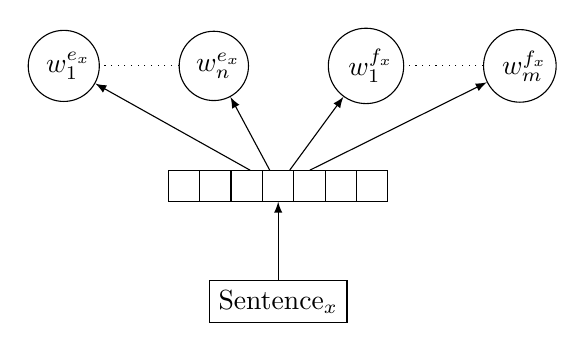
\begin{tikzpicture}[>=latex] 
\node[embedding] (Sx) {Sentence$_x$};
\node[hidden] (h1)[above=of Sx]{} edge [<-] (Sx);
\node[index] (We1) [above left =of h1] {$w^{e_x}_1$} edge [<-] (h1);
\node[index] (Wen) [right =of We1] {$w^{e_x}_n$}edge [<-] (h1) edge [ dotted ] (We1);
\node[index] (Wf1) [right =of Wen] {$w^{f_x}_1$}edge [<-] (h1) ;
\node[index] (Wfm) [right =of Wf1] {$w^{f_x}_m$}edge [<-] (h1) edge [ dotted ] (Wf1);
\end{tikzpicture}
\caption{Bilingual {\tt PV-DBOW}}
\label{f:bilingual_dbow}
\end{figure}





%\section{Introduction}
%....

\bibliographystyle{chicago}
\bibliography{bibliography}

\end{document}

%\begin{abstract}
%
%By representing the meaning of language in a vector space, we can model many semantic phenomena in a natural way.
%These representations have also proven useful for many Natural Language Processing tasks.
%We propose a method for using multilingual sentence embeddings to construct word embeddings in a shared vector space.
%We also highlight the difference between approaches that rely on local word context and on co-occurrence within sentences.
%Our model learns word embeddings that share features across multiple languages.
%We evaluate our word embeddings on a cross-lingual document classification task on two corpora.
%
%
%\end{abstract}
